\documentclass[10pt]{beamer}
\setbeamerfont{normal text}{size=\small}
\AtBeginDocument{\usebeamerfont{normal text}}

\usefonttheme{professionalfonts}

\usetheme[progressbar=frametitle]{metropolis}
\usepackage{appendixnumberbeamer}

\usepackage{booktabs}
\usepackage[scale=2]{ccicons}

\usepackage{pgfplots}
\usepgfplotslibrary{dateplot}

\usepackage{xspace}
\newcommand{\themename}{\textbf{\textsc{metropolis}}\xspace}

\title{Gatsby Bridging Program}
\subtitle{Probability: Discrete Distributions}
% \date{\today}
\date{}
\author{Cameron Stewart}
\institute{Gatsby Computational Neuroscience Unit}
\titlegraphic{\hfill
\includegraphics[height=1.5cm]{logo.png}}

\begin{document}

\maketitle

\begin{frame}{Table of contents}
  \setbeamertemplate{section in toc}[sections numbered]
  \tableofcontents%[hideallsubsections]
\end{frame}

\section{Random Variables, Probability Mass Functions, and Cumulative Distribution Functions}

\begin{frame}[fragile]{What is a Random Variable?}
Random variables are functions which map the possible outcomes of an experiment to numerical values. How we define these functions is up to us. In general, for random variable \(X\) and sample space \(\Omega\), we have that \(X: \Omega \rightarrow \mathbb{R}\).
\onslide<2>{\metroset{block=fill}\begin{exampleblock}{Example 1}
Consider a bag containing 3 red balls (R) and 5 green balls (G). In our experiment, we are going to draw 2 balls from the bag, with replacement. The sample space is \(\Omega = \left\{\text{RR}, \text{RG}, \text{GR}, \text{GG}\right\}\).

We are interested in determining the probabilities of drawing various numbers of red balls. To do this, we could start by defining a random variable \(X: \Omega \rightarrow \left\{0, 1, 2\right\}\) such that
\begin{equation*}
    X\left(\omega\right) =
    \begin{cases}
        0 & \text{if } \omega = \text{GG}\\
        1 & \text{if } \omega \in \left\{\text{RG, GR}\right\}\\
        2 & \text{if } \omega = \text{RR}
    \end{cases}\,.
\end{equation*}
\end{exampleblock}}
\end{frame}

\begin{frame}[fragile]{What is a Random Variable?}
Random variables are often utilised without any explicit reference to the sample space. Instead of writing \(X\left(\omega\right)\), we will typically just write \(X\). Instead of writing \(\mathbb{P}\left(E\right)\) for some event \(E\), we typically write \(\mathbb{P}\left(X \in A\right)\) for some set of numerical values \(A\).
\onslide<2>{\metroset{block=fill}\begin{exampleblock}{Example 1 Cont.}
What is the probability of drawing one red ball? We could express this as \(\mathbb{P}\left(\left\{\text{RG, GR}\right\}\right)\), but it is common and accepted notation to instead write \(\mathbb{P}\left(X \in \left\{1\right\}\right)\), or \(\mathbb{P}\left(0 < X < 2\right)\), or most preferably in this case \(\mathbb{P}\left(X = 1\right)\).
\begin{align*}
    \mathbb{P}\left(X = 1\right) &= \frac{3}{8}\frac{5}{8} + \frac{5}{8}\frac{3}{8}\\
    &= \frac{15}{32}\,.
\end{align*}
\end{exampleblock}}
\end{frame}

\begin{frame}[fragile]{The Chain Rule and Independence}
In a previous lecture, we covered the following relationship for events \(E\) and \(F\):
\begin{align*}
    \mathbb{P}\left(E \cap F\right) &= \mathbb{P}\left(E \mid F\right)\mathbb{P}\left(F\right)\\
    &= \mathbb{P}\left(F \mid E\right)\mathbb{P}\left(E\right)\,.
\end{align*}
\onslide<2->{This also applies to random variables. Here we are looking at the probability of random variables \(X\) and \(Y\) taking values in sets \(A\) and \(B\) respectively:
\metroset{block=fill}\begin{alertblock}{Chain Rule for Two Random Variables}
\begin{align*}
    \overbrace{\mathbb{P}\left(X \in A, Y \in B\right)}^{\text{Joint Prob.}} &= \overbrace{\mathbb{P}\left(X \in A \mid Y \in B\right)}^{\text{Conditional Prob.}}\overbrace{\mathbb{P}\left(Y \in B\right)}^{\text{Marginal Prob.}}\\
    &= \mathbb{P}\left(Y \in B \mid X \in A\right)\mathbb{P}\left(X \in A\right)
\end{align*}
\end{alertblock}}
\onslide<3>{A future lecture will cover joint, conditional, and marginal distributions and the chain rule, independence, and marginalisation in more detail.}
\end{frame}

\begin{frame}[fragile]{The Chain Rule and Independence}
In this lecture, we will only consider independent random variables. For two random variables to be independent, the realisation of one must have no effect on the distribution of the other. E.g. a coin flip is independent of the outcome of the previous coin flip.\onslide<2->{ Mathematically, we write this as
\begin{equation*}
    \mathbb{P}\left(X \in A, Y \in B\right) = \mathbb{P}\left(X \in A\right)\mathbb{P}\left(Y \in B\right)\,,
\end{equation*}
taking note that independence implies
\begin{equation*}
    \mathbb{P}\left(X \in A \mid Y \in B\right) = \mathbb{P}\left(X \in A\right)\,.
\end{equation*}}
\onslide<3>{For \(N\) independent random variables, this generalises to:
\metroset{block=fill}\begin{alertblock}{Independence of \(N\) Random Variables}
\begin{equation*}
    \mathbb{P}\left(X_1 \in A_1, \dots, X_N \in A_N\right) = \prod_{n=1}^N\mathbb{P}\left(X_n \in A_n\right)
\end{equation*}\end{alertblock}}
\end{frame}

\begin{frame}[fragile]{The Chain Rule and Independence}
\metroset{block=fill}\begin{exampleblock}{Example 1 Cont.}
In our red ball example, we could also use separate random variables for the outcomes of each draw from the bag. Let \(X_1 \in \left\{0, 1\right\}\) be the random variable representing the first draw and \(X_2 \in \left\{0, 1\right\}\) be the random variable representing the second draw (0 for a green ball and 1 for red ball). Then it is straightforward to see that \(X = X_1 + X_2\).

\onslide<2->{Are \(X_1\) and \(X_2\) independent?}\onslide<3->{ Yes, they are independent random variables, as the first draw has no effect on the second draw.}

\onslide<4->{What if we had the same experimental setup, but without replacing the ball after the first draw?}\onslide<5>{ In this case they are not independent, as the colour of the first drawn ball will dictate the probabilities of the second drawn ball.}
\end{exampleblock}
\end{frame}

\begin{frame}[fragile]{Discrete and Continuous Random Variables}
Discrete random variables can take a countable number of values. For example:
\begin{itemize}
    \item \(X \in \left\{0, 1\right\}\)
    \item \(X \in \left\{0, 1, 2, \dots\right\}\)
    \item \(X\) representing the number of buses arriving within an hour.
\end{itemize}

\onslide<2>{Continuous random variables can take values in continuous ranges. For example:
\begin{itemize}
    \item \(X \in \left[0, 1\right]\)
    \item \(X \in \mathbb{R}\)
    \item \(X\) representing the waiting time until the next bus.
\end{itemize}}
\end{frame}

\begin{frame}[fragile]{Probability Mass Functions}
Discrete distributions can be defined by their probability mass function (PMF). The PMF of random variable \(X\) is often denoted by \(f_X\) or \(p_X\), and is defined as:
\metroset{block=fill}\begin{alertblock}{Probability Mass Functions}
\begin{equation*}
    f_X\left(x\right) = \mathbb{P}\left(X = x\right)
\end{equation*}
\end{alertblock}
\onslide<2>{\(f_X\) is simply a function name. It is fine to use a different name, as long as it is clear how the function is defined. Occasionally, the same name is used for PMFs if it is clear from context how these are defined, but I'd advise against this practice for the sake of clarity. E.g. it is clearer to write \(p_X\left(x\right)\) and \(p_Y\left(y\right)\) than \(p\left(x\right)\) and \(p\left(y\right)\) if these correspond to 2 different PMFs.}
\end{frame}

\begin{frame}[fragile]{Probability Mass Functions}
Probabilities can't be negative and must sum to 1 over the set of all possible values \(\mathcal{X}\), so we have the following constraints:
\begin{equation*}
    f_X\left(x\right) \geq 0 \text{ for all } x
\end{equation*}
and
\begin{equation*}
    \sum_{x \in \mathcal{X}} f_X\left(x\right) = 1\,.
\end{equation*}
\(\mathcal{X}\) is referred to as the support of \(X\). \(f_X\left(x\right) = 0\) for \(x \notin \mathcal{X}\).
\end{frame}

\begin{frame}[fragile]{Probability Mass Functions}
\metroset{block=fill}\begin{exampleblock}{Example 1 Cont.}
Let's continue with our red ball example. What is the PMF of \(X\)? First, we recognise that \(\mathcal{X} = \left\{0, 1, 2\right\}\). You can verify for yourself that
\begin{equation*}
    f_X\left(x\right) =
    \begin{cases}
        \frac{25}{64} & \text{if } x = 0\\
        \frac{15}{32} & \text{if } x = 1\\
        \frac{9}{64} & \text{if } x = 2\\
        0 & \text{otherwise}
    \end{cases}\,,
\end{equation*}
and that this function satisfies the conditions for a PMF on the previous slide.
\end{exampleblock}
\end{frame}

\begin{frame}[fragile]{Probability Mass Functions}
Often, we use a \(\sim\) to mean "is distributed as". It is very common to see the notation
\begin{equation*}
    X \sim f_x\,,
\end{equation*}
which, in the discrete case, means that \(X\) has the PMF \(f_x\). Variations of this notation exist, but there should never be any ambiguity about the distribution of a random variable when using a \(\sim\).

\onslide<2>{Sometimes you will see
\begin{equation*}
    X_1, \dots, X_N \overset{\text{i.i.d.}}{\sim} f_x\,,
\end{equation*}
which implies that all \(N\) random variables are independent and identically distributed (i.i.d.) with PMF \(f_x\).}
\end{frame}

\begin{frame}[fragile]{Cumulative Distribution Functions}
A probability distribution can also be defined in terms of its cumulative distribution function (CDF). The CDF of a random variable \(X\) is a monotonically increasing function defined as:
\metroset{block=fill}\begin{alertblock}{Cumulative Distribution Functions}
\begin{equation*}
    F_X\left(x\right) = \mathbb{P}\left(X \leq x\right)
\end{equation*}
\end{alertblock}
\onslide<2>{For discrete random variables, we can relate this definition to the PMF as follows:
\begin{equation*}
    F_X\left(x\right) = \sum_{y\leq x} f_X\left(y\right)\,.
\end{equation*}}
\end{frame}

\begin{frame}[fragile]{Cumulative Distribution Functions}
As probabilities must sum to 1 over the support, we have the following emergent properties for CDFs:
\begin{align*}
    \lim_{x\rightarrow-\infty}F_X\left(x\right) = 0\\
    \lim_{x\rightarrow\infty}F_X\left(x\right) = 1
\end{align*}
\onslide<2>{We can also see that the following is true:
\begin{equation*}
    \mathbb{P}\left(a < X \leq b\right) = F_X\left(b\right) - F_X\left(a\right)\,.
\end{equation*}}
\end{frame}

\begin{frame}[fragile]{Cumulative Distribution Functions}
\metroset{block=fill}\begin{exampleblock}{Example 1 Cont.}
Back to the red ball example. What is the CDF of \(X\)? Previously, we found that
\begin{equation*}
    f_X\left(x\right) =
    \begin{cases}
        \frac{25}{64} & \text{if } x = 0\\
        \frac{15}{32} & \text{if } x = 1\\
        \frac{9}{64} & \text{if } x = 2\\
        0 & \text{otherwise}
    \end{cases}\,.
\end{equation*}
Hence, the CDF is
\begin{equation*}
    F_X\left(x\right) =
    \begin{cases}
        0 & \text{if } x < 0\\
        \frac{25}{64} & \text{if } 0 \leq x < 1\\
        \frac{55}{64} & \text{if } 1 \leq x < 2\\
        1 & \text{if } x \geq 2
    \end{cases}\,.
\end{equation*}
\end{exampleblock}
\end{frame}

\begin{frame}[fragile]{PDF and CDF Plots}
\metroset{block=fill}\begin{exampleblock}{Example 1 Cont.}
\begin{columns}
\begin{column}{0.425\textwidth}
\begin{figure}
    \centering
    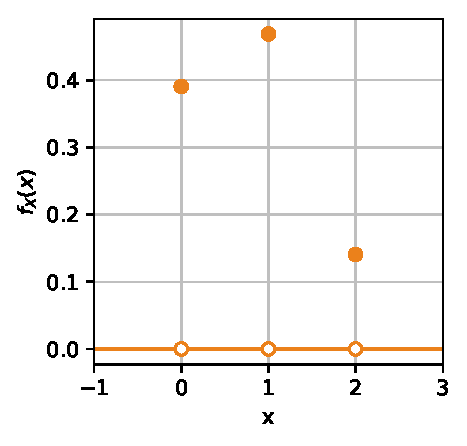
\includegraphics[width=\textwidth]{pmf.eps}
    \caption{Probability Mass Function}
\end{figure}
\end{column}
\begin{column}{0.425\textwidth}
\begin{figure}
    \centering
    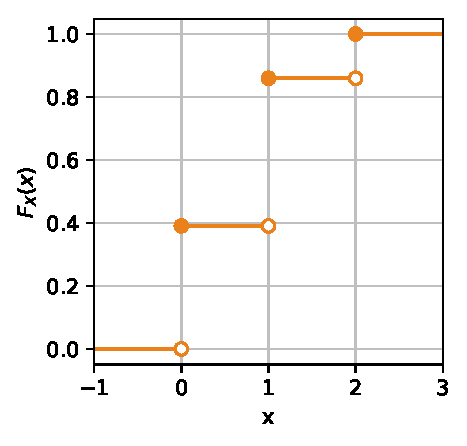
\includegraphics[width=\textwidth]{cdf.eps}
    \caption{Cumulative Distribution Function}
\end{figure}
\end{column}
\end{columns}
\end{exampleblock}
\end{frame}

\begin{frame}[fragile]{Sampling}
Similarly to how we refer to realisations of random variables, we can also talk about samples of distributions. Sampling from a discrete distribution with PMF \(f_x\) simply implies that we randomly generate a number \(x\) with probability \(f_x\left(x\right)\).

\onslide<2->{To be entirely correct, drawing \(N\) samples from \(f_x\) involves running \(N\) random experiments with \(N\) associated random variables \(X_1, \dots, X_N \overset{\text{i.i.d.}}{\sim} f_x\) and generating \(N\) realisations \(x_1, \dots, x_N\).}

\onslide<3>{As \(N \rightarrow \infty\), we will observe that
\begin{equation*}
    \frac{\sum_{n = 1}^N \href{https://en.wikipedia.org/wiki/Iverson_bracket}{\color{mLightBrown}{\left[x_n = x\right]}}}{N} \rightarrow f_x\left(x\right)
\end{equation*}}
\end{frame}

\begin{frame}[standout]
Intermission
\end{frame}

\section{Expectation and Variance}

\begin{frame}[fragile]{Expectations}
Suppose we want to know the average value of a function \(g\left(x\right)\) evaluated at samples from a distribution. More precisely, we wish to draw realisations of \(X_1, \dots, X_N \overset{\text{i.i.d.}}{\sim} f_x\) and then compute the mean of \(\left\{g\left(x_1\right), \dots, g\left(x_N\right)\right\}\). As \(N\) increases, this will converge to a value which we call the expectation (or expected value). This theorem is referred to as the law of large numbers.

We can estimate the expectation for finite \(N\) as follows:
\metroset{block=fill}\begin{alertblock}{Empirical Estimates of Expectations}
\begin{equation*}
    \underset{X \sim f_X}{\mathbb{E}}\left[g\left(X\right)\right] \approx \frac{1}{N}\sum_{n = 1}^N g\left(x_n\right)\qquad\text{for large }N
\end{equation*}
\end{alertblock}
\end{frame}

\begin{frame}[fragile]{Expectations}
If \(X\) is discrete with support \(\mathcal{X}\) and PMF \(f_X\), we can also define this expectation as a weighted average:
\metroset{block=fill}\begin{alertblock}{Expectations on Discrete Distributions}
\begin{equation*}
    \underset{X \sim f_X}{\mathbb{E}}\left[g\left(X\right)\right] = \sum_{x \in \mathcal{X}} f_X\left(x\right)g\left(x\right)
\end{equation*}
\end{alertblock}
If the distribution on which the expectation is taken is clear from context, the text under the \(\mathbb{E}\) is often omitted.
\end{frame}

\begin{frame}[fragile]{Rules for Expectations}
\begin{itemize}
    \item Linearity:
        \begin{equation*}
            \mathbb{E}\left[ag\left(X\right) + bh\left(X\right)\right] = a\mathbb{E}\left[g\left(X\right)\right] + b\mathbb{E}\left[h\left(X\right)\right]\,,
        \end{equation*}
        for constants \(a, b\) and functions \(g, h\).
    \item Non-multiplicativity:
        In general
        \begin{equation*}
            \mathbb{E}\left[g\left(X\right)h\left(X\right)\right] \neq \mathbb{E}\left[g\left(X\right)\right]\mathbb{E}\left[h\left(X\right)\right]\,.
        \end{equation*}
    \item Multiplicativity under independence:
        If \(X_1, \dots, X_N\) are independent, then
        \begin{equation*}
            \mathbb{E}\left[\prod_{n=1}^N g_n\left(X_n\right)\right] = \prod_{n=1}^N\mathbb{E}\left[g_n\left(X_n\right)\right]\,,
        \end{equation*}
        for functions \(g_n\). The definition of a multivariate expectation will make more sense in later lectures when multivariate distributions are covered.
\end{itemize}
\end{frame}

\begin{frame}[fragile]{Expectations}
\metroset{block=fill}\begin{exampleblock}{Example 2}
    Suppose we roll 2 dice. Let \(X_1\) and \(X_2\) represent the first and second roll respectively.
\end{exampleblock}
\end{frame}

\begin{frame}[standout]
Intermission
\end{frame}

\section{Common Discrete Distributions}

\begin{frame}[standout]
Intermission
\end{frame}

\section{Introduction to Stochastic Processes}


















% \section[Intro]{Introduction}

% \begin{frame}[fragile]{Metropolis}

%   The \themename theme is a Beamer theme with minimal visual noise
%   inspired by the \href{https://github.com/hsrmbeamertheme/hsrmbeamertheme}{\textsc{hsrm} Beamer
%   Theme} by Benjamin Weiss.

%   Enable the theme by loading

%   \begin{verbatim}    \documentclass{beamer}
%     \usetheme{metropolis}\end{verbatim}

%   Note, that you have to have Mozilla's \emph{Fira Sans} font and XeTeX
%   installed to enjoy this wonderful typography.
% \end{frame}
% \begin{frame}[fragile]{Sections}
%   Sections group slides of the same topic

%   \begin{verbatim}    \section{Elements}\end{verbatim}

%   for which \themename provides a nice progress indicator \ldots
  
% \end{frame}

% \section{Titleformats}

% \begin{frame}{Metropolis titleformats}
% 	\themename supports 4 different titleformats:
% 	\begin{itemize}
% 		\item Regular
% 		\item \textsc{Smallcaps}
% 		\item \textsc{allsmallcaps}
% 		\item ALLCAPS
% 	\end{itemize}
% 	They can either be set at once for every title type or individually.
% \end{frame}

% \subsection{Tricks}

% {
%     \metroset{titleformat frame=smallcaps}
% \begin{frame}{Small caps}
% 	This frame uses the \texttt{smallcaps} titleformat.

% 	\begin{alertblock}{Potential Problems}
% 		Be aware, that not every font supports small caps. If for example you typeset your presentation with pdfTeX and the Computer Modern Sans Serif font, every text in smallcaps will be typeset with the Computer Modern Serif font instead.
% 	\end{alertblock}
% \end{frame}
% }

% {
% \metroset{titleformat frame=allsmallcaps}
% \begin{frame}{All small caps}
% 	This frame uses the \texttt{allsmallcaps} titleformat.

% 	\begin{alertblock}{Potential problems}
% 		As this titleformat also uses smallcaps you face the same problems as with the \texttt{smallcaps} titleformat. Additionally this format can cause some other problems. Please refer to the documentation if you consider using it.

% 		As a rule of thumb: Just use it for plaintext-only titles.
% 	\end{alertblock}
% \end{frame}
% }

% {
% \metroset{titleformat frame=allcaps}
% \begin{frame}{All caps}
% 	This frame uses the \texttt{allcaps} titleformat.

% 	\begin{alertblock}{Potential Problems}
% 		This titleformat is not as problematic as the \texttt{allsmallcaps} format, but basically suffers from the same deficiencies. So please have a look at the documentation if you want to use it.
% 	\end{alertblock}
% \end{frame}
% }

% \section{Elements}

% \begin{frame}[fragile]{Typography}
%       \begin{verbatim}The theme provides sensible defaults to
% \emph{emphasize} text, \alert{accent} parts
% or show \textbf{bold} results.\end{verbatim}

%   \begin{center}becomes\end{center}

%   The theme provides sensible defaults to \emph{emphasize} text,
%   \alert{accent} parts or show \textbf{bold} results.
% \end{frame}

% \begin{frame}{Font feature test}
%   \begin{itemize}
%     \item Regular
%     \item \textit{Italic}
%     \item \textsc{SmallCaps}
%     \item \textbf{Bold}
%     \item \textbf{\textit{Bold Italic}}
%     \item \textbf{\textsc{Bold SmallCaps}}
%     \item \texttt{Monospace}
%     \item \texttt{\textit{Monospace Italic}}
%     \item \texttt{\textbf{Monospace Bold}}
%     \item \texttt{\textbf{\textit{Monospace Bold Italic}}}
%   \end{itemize}
% \end{frame}

% \begin{frame}{Lists}
%   \begin{columns}[T,onlytextwidth]
%     \column{0.33\textwidth}
%       Items
%       \begin{itemize}
%         \item Milk \item Eggs \item Potatos
%       \end{itemize}

%     \column{0.33\textwidth}
%       Enumerations
%       \begin{enumerate}
%         \item First, \item Second and \item Last.
%       \end{enumerate}

%     \column{0.33\textwidth}
%       Descriptions
%       \begin{description}
%         \item[PowerPoint] Meeh. \item[Beamer] Yeeeha.
%       \end{description}
%   \end{columns}
% \end{frame}
% \begin{frame}{Animation}
%   \begin{itemize}[<+- | alert@+>]
%     \item \alert<4>{This is\only<4>{ really} important}
%     \item Now this
%     \item And now this
%   \end{itemize}
% \end{frame}
% \begin{frame}{Figures}
%   \begin{figure}
%     \newcounter{density}
%     \setcounter{density}{20}
%     \begin{tikzpicture}
%       \def\couleur{alerted text.fg}
%       \path[coordinate] (0,0)  coordinate(A)
%                   ++( 90:5cm) coordinate(B)
%                   ++(0:5cm) coordinate(C)
%                   ++(-90:5cm) coordinate(D);
%       \draw[fill=\couleur!\thedensity] (A) -- (B) -- (C) --(D) -- cycle;
%       \foreach \x in {1,...,40}{%
%           \pgfmathsetcounter{density}{\thedensity+20}
%           \setcounter{density}{\thedensity}
%           \path[coordinate] coordinate(X) at (A){};
%           \path[coordinate] (A) -- (B) coordinate[pos=.10](A)
%                               -- (C) coordinate[pos=.10](B)
%                               -- (D) coordinate[pos=.10](C)
%                               -- (X) coordinate[pos=.10](D);
%           \draw[fill=\couleur!\thedensity] (A)--(B)--(C)-- (D) -- cycle;
%       }
%     \end{tikzpicture}
%     \caption{Rotated square from
%     \href{http://www.texample.net/tikz/examples/rotated-polygons/}{texample.net}.}
%   \end{figure}
% \end{frame}
% \begin{frame}{Tables}
%   \begin{table}
%     \caption{Largest cities in the world (source: Wikipedia)}
%     \begin{tabular}{lr}
%       \toprule
%       City & Population\\
%       \midrule
%       Mexico City & 20,116,842\\
%       Shanghai & 19,210,000\\
%       Peking & 15,796,450\\
%       Istanbul & 14,160,467\\
%       \bottomrule
%     \end{tabular}
%   \end{table}
% \end{frame}
% \begin{frame}{Blocks}
%   Three different block environments are pre-defined and may be styled with an
%   optional background color.

%   \begin{columns}[T,onlytextwidth]
%     \column{0.5\textwidth}
%       \begin{block}{Default}
%         Block content.
%       \end{block}

%       \begin{alertblock}{Alert}
%         Block content.
%       \end{alertblock}

%       \begin{exampleblock}{Example}
%         Block content.
%       \end{exampleblock}

%     \column{0.5\textwidth}

%       \metroset{block=fill}

%       \begin{block}{Default}
%         Block content.
%       \end{block}

%       \begin{alertblock}{Alert}
%         Block content.
%       \end{alertblock}

%       \begin{exampleblock}{Example}
%         Block content.
%       \end{exampleblock}

%   \end{columns}
% \end{frame}
% \begin{frame}{Math}
%   \begin{equation*}
%     e = \lim_{n\to \infty} \left(1 + \frac{1}{n}\right)^n
%   \end{equation*}
% \end{frame}
% \begin{frame}{Line plots}
%   \begin{figure}
%     \begin{tikzpicture}
%       \begin{axis}[
%         mlineplot,
%         width=0.9\textwidth,
%         height=6cm,
%       ]

%         \addplot {sin(deg(x))};
%         \addplot+[samples=100] {sin(deg(2*x))};

%       \end{axis}
%     \end{tikzpicture}
%   \end{figure}
% \end{frame}
% \begin{frame}{Bar charts}
%   \begin{figure}
%     \begin{tikzpicture}
%       \begin{axis}[
%         mbarplot,
%         xlabel={Foo},
%         ylabel={Bar},
%         width=0.9\textwidth,
%         height=6cm,
%       ]

%       \addplot plot coordinates {(1, 20) (2, 25) (3, 22.4) (4, 12.4)};
%       \addplot plot coordinates {(1, 18) (2, 24) (3, 23.5) (4, 13.2)};
%       \addplot plot coordinates {(1, 10) (2, 19) (3, 25) (4, 15.2)};

%       \legend{lorem, ipsum, dolor}

%       \end{axis}
%     \end{tikzpicture}
%   \end{figure}
% \end{frame}
% \begin{frame}{Quotes}
%   \begin{quote}
%     Veni, Vidi, Vici
%   \end{quote}
% \end{frame}

% {%
% \setbeamertemplate{frame footer}{My custom footer}
% \begin{frame}[fragile]{Frame footer}
%     \themename defines a custom beamer template to add a text to the footer. It can be set via
%     \begin{verbatim}\setbeamertemplate{frame footer}{My custom footer}\end{verbatim}
% \end{frame}
% }

% \begin{frame}{References}
%   Some references to showcase [allowframebreaks] \cite{knuth92,ConcreteMath,Simpson,Er01,greenwade93}
% \end{frame}

% \section{Conclusion}

% \begin{frame}{Summary}

%   Get the source of this theme and the demo presentation from

%   \begin{center}\url{github.com/matze/mtheme}\end{center}

%   The theme \emph{itself} is licensed under a
%   \href{http://creativecommons.org/licenses/by-sa/4.0/}{Creative Commons
%   Attribution-ShareAlike 4.0 International License}.

%   \begin{center}\ccbysa\end{center}

% \end{frame}

% {\setbeamercolor{palette primary}{fg=black, bg=yellow}
% \begin{frame}[standout]
%   Questions?
% \end{frame}
% }

% \appendix

% \begin{frame}[fragile]{Backup slides}
%   Sometimes, it is useful to add slides at the end of your presentation to
%   refer to during audience questions.

%   The best way to do this is to include the \verb|appendixnumberbeamer|
%   package in your preamble and call \verb|\appendix| before your backup slides.

%   \themename will automatically turn off slide numbering and progress bars for
%   slides in the appendix.
% \end{frame}

% \begin{frame}[allowframebreaks]{References}

%   \bibliography{demo}
%   \bibliographystyle{abbrv}

% \end{frame}

\end{document}
